\documentclass[12pt]{article}
\usepackage{graphicx}
\textwidth=7in
\textheight=9.5in
\topmargin=-1in
\headheight=0in
\headsep=.5in
\hoffset  -.85in

\pagestyle{empty}

\renewcommand{\thefootnote}{\fnsymbol{footnote}}
\begin{document}

\begin{center}
{\bf CS165 Database Systems  
\\ Homework 2 - PostgreSQL Table Definition
}
\end{center}

\setlength{\unitlength}{1in}

\begin{picture}(6,.1) 
\put(0,0) {\line(1,0){6.25}}         
\end{picture}

\vskip.25in
\noindent\textbf{Submission:} Sunday, November 31, 23:59:99, cs165.13.14.2@gmail.com

\vskip.25in
\noindent \textbf{Requirements}:
\vskip.15in 
\noindent A zip file containing the following items:
\begin{itemize}
  \item 2 SQL script file containing your table definitions.
  \item A readme.txt file explaining any design decisions you made in converting the ERDs to Postgres tables.
\end{itemize}
\noindent The zip file's name should be your student number (e.g. 2001-65721.zip).

\vskip.25in
\noindent \textbf{Problem}:
\vskip.15in
\noindent Consider the following ER Diagrams. For each diagram, write an SQL script file that will produce corresponding tables. In an accompanying readme file, indicate any design decisions you made. Also indicate any constraints you were unable to capture in your tables, and why you were unable to capture them. The following psql command can be used to read and execute all SQL statements inside an SQL script file (*.sql):

\vskip.15in 
\begin{verbatim}
	\i [file-path]
\end{verbatim}

\begin{figure}[h!]
  \caption{Music Store Customer Database}
  \centering
    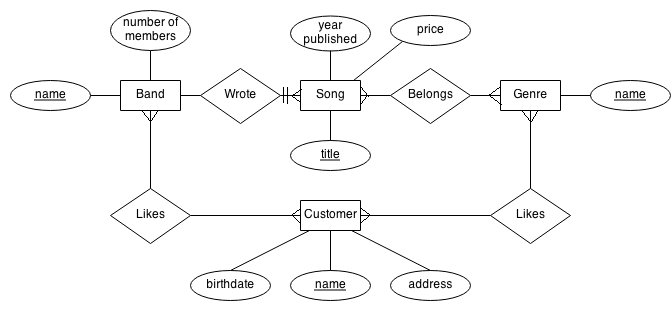
\includegraphics[width=1.0\textwidth]{01.png}
\end{figure}

\begin{figure}[h!]
  \caption{Employee Database}
  \centering
    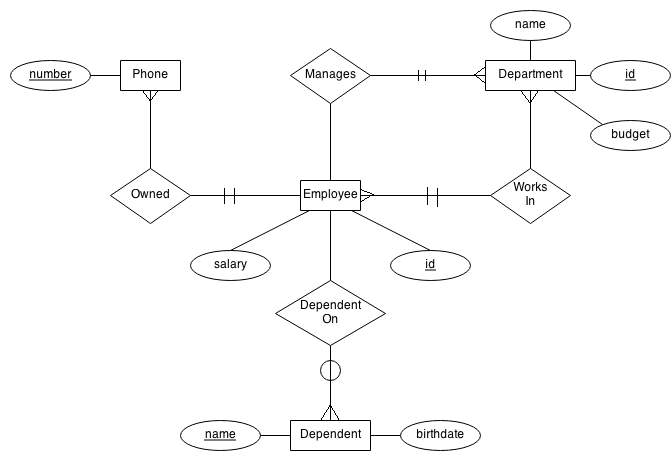
\includegraphics[width=1.0\textwidth]{02.png}
\end{figure}

\end{document}
